


\chapter{Observations}
  \label{ch_rbsp}

\todo{You know what would be great for putting this numerical work in context? A nice, consistent survey that breaks down the occurrence rate of Pc4 pulsations by harmonic, etc. }

\todo{There have been some surveys in the past. Dai did a nice one last year, but his filter biased him against the fundamental mode. And only a few past works have even worried about harmonic mode... probably because it's hard to get that information unless you have both E and B. }

\todo{Furthermore, it's awkward that Pgs are identified by visual inspection. How can we say how rare they are if they aren't rigorously defined? }

\todo{Probably need some fluff here with appropriate citations for the mission and the instrumentation. }

\todo{The tools used in the present chapter --- SPEDAS and the SPICE kernel --- are publicly available. They run best with an IDL license, which is not, but they are functional using just the (free) IDL virtual machine. The code is wrapped up in a Git repository: \url{https://github.com/chizarlicious/RBSP} (maybe should make a GitHub organization to hold this code, to decouple it from my personal account?). }



Past studies to compare to:

Anderson\cite{anderson_1990} located events by visual inspection of AMPTE/CCE data. He found that toroidal resonances outnumber poloidal ones about three-to-one. ``Harmonic toroidal resonances'' are spread 0600 to 1600. ``Fundamental toroidal resonances'' (which are not mutually exclusive with harmonic ones!) appear everywhere but dusk. Poloidal modes occur everywhere but dawn; odd and even harmonics are not distinguished. Notably, most observation time was spent at $L > 7$. Orbit near the equator, magnetic field instrumentation, so fundamental poloidal modes would have been hard to observe. 

Dai\cite{dai_2015} found 890 poloidal Pc4 events using RBSP. Due to a cutoff in magnetic field amplitude, his findings are also biased in favor of the even mode. Events are shown to be most common near noon, but smeared across the dayside, and with a few odd stragglers near midnight. Low-\azm waves were shown to be smeared a bit more, occurring across the entire dusk flank at low rates. 

Motoba\cite{motoba_2015} looked specifically at giant pulsations -- 105 events. Seen from midnight to noon, with a strong peak before dawn, 0300 or so. 

%Observations show that the poloidal mode is most excited in the second harmonic\cite{cummings_1969,hughes_1978,arthur_1981,singer_1982,takahashi_1984,engebretson_1988} even when there is a strong compressional component\cite{takahashi_1987,haerendel_1999,vaivads_2001,sibeck_2012}. 

% -----------------------------------------------------------------------------
% -----------------------------------------------------------------------------
% -----------------------------------------------------------------------------
\section{Sampling Bias and Event Selection}
  \label{sec_selection}

The present analysis makes use of as much Van Allen Probe data as is available at the time of writing: October 2012 to August 2015. Between the two probes, that's just over 2000 days of observation. 

Notably, the two probes are taken to be independent observers. The vast majority of Pc4 observations take place near apogee, where the probes are separated by several hours. Pc4 pulsations tend to be localized in MLT --- indeed, this was a key justification for the model described in \cref{ch_model}. The two probes simultaneously observe the same event only \todo{$\cdots$} of the time. 

\todo{How common is it for one probe to see an event, then the other probe to fly through that same event an hour or two later? }

Electric and magnetic waveform data is cleaned up by averaging over the probe's spin period, \SI{10.5}{\s}. The three-dimensional electric field is then obtained using the assumption $\vec{E} \cdot \vec{B} = 0$. Notably, this assumption is taken only when the probe's spin plane is offset from the magnetic field by at least \SI{15}{\degree}. The rest of the data --- about half --- is discarded, which introduces a sampling bias against the flanks. 

A further bias is introduced by the probes' non-integer number of precessions around Earth. Pc4 pulsations are most commonly observed near apogee. As of July 2014, apogee had precessed once around Earth\cite{dai_2015}. The present work considers roughly one and a half precessions; the nightside has been sampled at apogee twice as often as the dayside. 

The spatial distribution of usable data --- that is, data for which three-dimensional electric and magnetic fields are abailable --- is shown in \cref{fig_pos_all_sharp}. Bins are unitary in $L$ (divided at integer $L$) and in MLT (centered at integer hours). Event distribution in magnetic latitude is not shown; the Van Allen Probes are localized to within \todo{\SI{15}{\degree}} of the equatorial plane. 

\todo{$L$ is italicized and MLT is not? That seems weird. }

\begin{figure}[!htb]
    \centering
    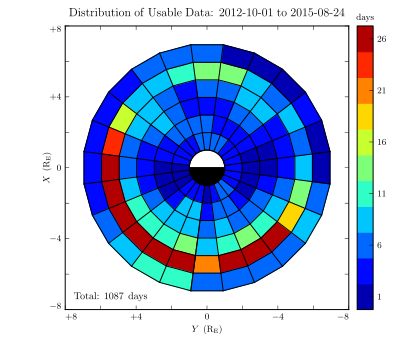
\includegraphics[width=\textwidth]{figures/pos_all_sharp.pdf}
    \caption[Distribution of Usable Van Allen Probe Data: Fine Resolution]{
      Three-dimensional electric field values are computed by assuming $\vec{E} \cdot \vec{B} = 0$. Data is discarded whenever the magnetic field falls within \SI{15}{\degree} of the spin plane, which introduces a bias against the flanks. Furthermore, the probes have completed only one and a half precessions around Earth; the dayside has been sampled once at apogee, and the nightside twice. 
    }
    \label{fig_pos_all_sharp}
\end{figure}

Awkwardly, coverage is weakest from pre-dawn to the mid-afternoon --- the exact regions where Pc4 pulsations have been shown to peak. In order to compensate for that fact, results in the present chapter are binned coarsely. Histogram bins are two hours wide in MLT. Only two bins are used in the radial direction: $L \leq 5$ and $L > 5$. 

\todo{Most events occur between $L = 4$ and $L = 6$, but splitting at $L = 5$ is otherwise arbitrary. It might make more sense to split the bins wherever the median event is or something. }

\todo{Show all sampling together? Show two plots, based on Dst? Showing it all, as is presently done, seems like overkill. }

\begin{figure}[!htb]
    \centering
    \includegraphics[width=\textwidth]{figures/pos_all.pdf}
    \caption[Distribution of Usable Van Allen Probe Data]{
      \todo{This is the sampling distribution used to normalize Dst-agnostic event counts. It's not clear that all of these plots are necessary. }
    }
    \label{fig_pos_all}
\end{figure}

\begin{figure}[!htb]
    \centering
    \includegraphics[width=\textwidth]{figures/pos_storm.pdf}
    \caption[Distribution of Usable Van Allen Probe Data: Dst$\geq \SI{-30}{\nT}$]{
      \todo{This is the sampling distribution used to normalize event counts at Dst$\geq \SI{-30}{\nT}$. It's not clear that all of these plots are necessary. }
    }
    \label{fig_pos_calm}
\end{figure}


\begin{figure}[!htb]
    \centering
    \includegraphics[width=\textwidth]{figures/pos_storm.pdf}
    \caption[Distribution of Usable Van Allen Probe Data: Dst $< \SI{-30}{\nT}$]{
      \todo{This is the sampling distribution used to normalize event counts at Dst$< \SI{-30}{\nT}$. It's not clear that all of these plots are necessary. }
    }
    \label{fig_pos_storm}
\end{figure}

Field measurements are transformed from GSE coordinates into the same dipole coordinates used in \cref{ch_model,ch_results}. The \z axis is parallel to the background magnetic field, which is estimated using a ten-minute running average of the magnetic field measurements. The \y axis is defined per $\yhat \parallel \zhat \times \vec{r}$. The \x axis is then defined per $\xhat \equiv \yhat \times \zhat$. This method is described by Liu\cite{liu_2010}, and guarantees that the axes are right-handed and pairwise orthogonal. 

The \about1000 days of usable data are considered half an hour at a time --- \about60 data points per event at the ten-second spinfit cadence. This allows for a frequency resolution of \about\SI{0.5}{\mHz} in the discrete Fourier transform. Spectra are computed for all six field components: \dft{B_x}, \dft{B_y}, \dft{B_z}, \dft{E_x}, \dft{E_y}, and \dft{E_z}. 

The background magnetic is subtracted off before performing each transform, leaving only the magnetic field perturbation along each axis. (As in \cref{ch_model,ch_results}, $B_x$ refers not to the full magnetic field in the \x direction, but to its perturbation from the zeroth-order field.) Each waveform is also shifted horizontally so that its mean over the thirty minute event is zero. 

Frequency-domain Poynting flux is computed from the electric and magnetic field transforms. Values are effective at the ionosphere; a factor of $L^3$ is introduced to account for the compression of the flux tube. Poloidal and toroidal Poynting flux, respectively, are given by:
\begin{align}
  \dft{S_P} &\equiv -\frac{L^3}{\mz} \dft{E_y} \dft{B_x^*} &
  \dft{S_T} &\equiv  \frac{L^3}{\mz} \dft{E_x} \dft{B_y^*}
\end{align}

\todo{The Poynting flux scaled by $L^3$ to conserve energy. But doesn't the magnetic field be scale with $L^3$ to conserve flux, and the electric field scale with the magnetic field? }

The Poynting fluxes $\dft{S}$ for each event are filtered based on frequency, magnitude, and phase offset. The poloidal and toroidal channels are checked independently; a given half hour can have no event, a poloidal event, a toroidal event, or both. 

A Gaussian profile is fit to $|\mathbb{I}\mathrm{m}\dft{S}|$, which corresponds to the magnitude of the standing wave (in turn, the real component is the traveling wave). If the fit fails, for example due to non-finite values in the data, the event is discarded. The event is also discarded if the peak of the Gaussian does not correspond to the largest spectral feature in the data, standing or traveling; that is, the event is disqualified if the Gaussian is not centered within \SI{5}{\mHz} of the maximum value of $|\dft{S}|$. 

Non-Pc4 events are filtered out: any event for which the standing wave Gaussian does not fall in the range \SIrange{7}{25}{\mHz}. Notably, no filter is imposed on spectral width. 

Out of consideration for instrument sensitivity, events are thresholded at a magnitude of $|\mathbb{I}\mathrm{m}\dft{S}| \geq \SI{e-2}{\mW/\m\squared}$. 

Events are filtered based on the phase offset between the electric and magnetic field waveforms, given by $\arctan\frac{ \mathbb{I}\mathrm{m}\dft{S} }{ \mathbb{R}\mathrm{e}\dft{S} }$. For a purely traveling wave, the electric and magnetic field waveforms are in phase (\SI{0}{\degree}) or in antiphase (\SI{180}{\degree}). Standing waves have a phase of $\pm\SI{90}{\degree}$ between their electric and magnetic field components. The events presented here are filtered conservatively in phase; the standing wave must just barely exceed the traveling wave (phase between \SI{45}{\degree} and \SI{135}{\degree} in absolute value). 

Events are filtered on coherence, to ensure that the phase offset is credible. If the coherence between \dft{E} and \dft{B^*} is less than 0.9, the event is discarded. Coherence and phase are both measured at the discrete Fourier transform point closest to the peak of the Gaussian. 

Finally, any event within \SI{3}{\degree} of the magnetic equator is discarded due to ambiguity in its phase. As discussed in \cref{ch_flrs}, odd and even harmonics are distinguished by the sign of the phase offset between the electric and magnetic field. For example, in odd poloidal modes, an observer north of the equator sees $B_x$ lead $E_y$ by a phase of \SI{90}{\degree}, and an observer below the equator sees the opposite. When the probe is very close to the equator, an event's parity becomes ambiguous. 

\todo{We try not to worry too much about first vs third harmonic, since we can't tell them apart except by guessing at frequency. Chisham and Orr\cite{chisham_1991} argue that around \SI{7}{\RE}, frequency around \SI{10}{\mHz} precludes higher harmonics. Or maybe look at \cite{green_1985}? }

% -----------------------------------------------------------------------------
% -----------------------------------------------------------------------------
% -----------------------------------------------------------------------------
\section{Overall Rate of Pc4 Events}
  \label{sec_total}

\begin{figure}[!htb]
    \centering
    \includegraphics[width=\textwidth]{figures/rate_all.pdf}
    \caption[Pc4 Rate]{
      \todo{Pc4s are observed at all local times, but are most common near noon and least common near dusk. }
    }
    \label{fig_rate_all}
\end{figure}

\begin{figure}[!htb]
    \centering
    \includegraphics[width=\textwidth]{figures/rate_calm.pdf}
    \caption[Pc4 Rate: Dst$\geq \SI{-30}{\nT}$]{
      \todo{$\cdots$}
    }
    \label{fig_rate_calm}
\end{figure}

\begin{figure}[!htb]
    \centering
    \includegraphics[width=\textwidth]{figures/rate_storm.pdf}
    \caption[Pc4 Rate: Dst$< \SI{-30}{\nT}$]{
      \todo{During geomagnetically active times, Pc4 pulsations become much more common on the dayside. }
    }
    \label{fig_rate_storm}
\end{figure}

\begin{figure}[!htb]
    \centering
    \includegraphics[width=\textwidth]{figures/rate_all_lpp.pdf}
    \caption[Pc4 Rate Inside and Outside the Plasmapause]{
      \todo{Almost all Pc4 events are outside the plasmapause. }
    }
    \label{fig_rate_all_lpp}
\end{figure}

% -----------------------------------------------------------------------------
% -----------------------------------------------------------------------------
% -----------------------------------------------------------------------------
\section{Pc4 Events by Mode}
  \label{sec_mode}

The filters described in \cref{sec_selection} yield 822 events: 136 odd poloidal modes, 234 even poloidal modes, 445 odd toroidal modes, and 86 even toroidal modes. The distributions of those events are shown in \cref{fig_mode_all,fig_mode_storm}; counts are normalized to the sampling rates shown in \cref{fig_pos_all,fig_pos_storm} respectively. 

\todo{Get a better handle on the numbers presented by Anderson\cite{anderson_1990}. That was ground, based, I think, and the categorization was really inconvenient. }

\todo{It's good to see that even poloidal and even toroidal modes have similar distributions, since one turns into the other. The relationship is less clear for the odd modes, but odd poloidal and odd toroidal events are both least common near dusk. }

\todo{Odd toroidal events are by far the most commonly observed. }

\todo{Even modes are less likely to be observed on the ground? \cite{takahashi_1992} }

\begin{figure}[!htb]
    \centering
    \includegraphics[width=\textwidth]{figures/mode_all.pdf}
    \caption[Pc4 Rate by Mode]{
      \todo{Even harmonics are strongly peaked at noon, with some presence smeared across the dusk side. Odd harmonics, on the other hand, are mostly seen on the dawn side. }
    }
    \label{fig_mode_all}
\end{figure}

\begin{figure}[!htb]
    \centering
    \includegraphics[width=\textwidth]{figures/mode_calm.pdf}
    \caption[Pc4 Rate by Mode: Dst$\geq \SI{-30}{\nT}$]{
      \todo{$\cdots$}
    }
    \label{fig_mode_calm}
\end{figure}

\begin{figure}[!htb]
    \centering
    \includegraphics[width=\textwidth]{figures/mode_storm.pdf}
    \caption[Pc4 Rate by Mode: Dst$< \SI{-30}{\nT}$]{
      \todo{Pc4 events near noon are much more common during geomagnetically active times. }
    }
    \label{fig_mode_storm}
\end{figure}

% -----------------------------------------------------------------------------
% -----------------------------------------------------------------------------
% -----------------------------------------------------------------------------
\section{Poloidal Pc4 Events by Compressional Coupling}

\todo{Low-\azm poloidal Pc4 events are coupled to the compressional mode, while high-\azm ones are not. }

\begin{figure}[!htb]
    \centering
    \includegraphics[width=\textwidth]{figures/azm_rate_all.pdf}
    \caption[Poloidal Pc4 Rate by Compressional Coupling]{
      \todo{Low-\azm poloidal Pc4 events are more common on the nightside than high-\azm events. }
    }
    \label{fig_azm_rate_all}
\end{figure}


\begin{figure}[!htb]
    \centering
    \includegraphics[width=\textwidth]{figures/azm_rate_calm.pdf}
    \caption[Poloidal Pc4 Rate by Compressional Coupling: Dst$\geq \SI{-30}{\nT}$]{
      \todo{$\cdots$}
    }
    \label{fig_azm_rate_calm}
\end{figure}


\begin{figure}[!htb]
    \centering
    \includegraphics[width=\textwidth]{figures/azm_rate_storm.pdf}
    \caption[Poloidal Pc4 Rate by Compressional Coupling: Dst$< \SI{-30}{\nT}$]{
      \todo{$\cdots$}
    }
    \label{fig_azm_rate_storm}
\end{figure}



% -----------------------------------------------------------------------------
% -----------------------------------------------------------------------------
% -----------------------------------------------------------------------------
\section{Pc4 Events by Spectral Width}


\begin{figure}[!htb]
    \centering
    \includegraphics[width=\textwidth]{figures/fwhm_rate_p_all.pdf}
    \caption[Poloidal Pc4 Rate by Compressional Coupling]{
      \todo{$\cdots$}
    }
    \label{fig_fwhm_rate_p_all}
\end{figure}

\begin{figure}[!htb]
    \centering
    \includegraphics[width=\textwidth]{figures/fwhm_rate_p_calm.pdf}
    \caption[Poloidal Pc4 Rate by Compressional Coupling: Dst$\geq \SI{-30}{\nT}$]{
      \todo{$\cdots$}
    }
    \label{fig_fwhm_rate_p_calm}
\end{figure}

\begin{figure}[!htb]
    \centering
    \includegraphics[width=\textwidth]{figures/fwhm_rate_p_storm.pdf}
    \caption[Poloidal Pc4 Rate by Compressional Coupling: Dst$< \SI{-30}{\nT}$]{
      \todo{$\cdots$}
    }
    \label{fig_fwhm_rate_p_storm}
\end{figure}

\begin{figure}[!htb]
    \centering
    \includegraphics[width=\textwidth]{figures/fwhm_rate_t_all.pdf}
    \caption[Toroidal Pc4 Rate by Compressional Coupling]{
      \todo{$\cdots$}
    }
    \label{fig_fwhm_rate_t_all}
\end{figure}

\begin{figure}[!htb]
    \centering
    \includegraphics[width=\textwidth]{figures/fwhm_rate_t_calm.pdf}
    \caption[Toroidal Pc4 Rate by Compressional Coupling: Dst$\geq \SI{-30}{\nT}$]{
      \todo{$\cdots$}
    }
    \label{fig_fwhm_rate_t_calm}
\end{figure}

\begin{figure}[!htb]
    \centering
    \includegraphics[width=\textwidth]{figures/fwhm_rate_t_storm.pdf}
    \caption[Toroidal Pc4 Rate by Compressional Coupling: Dst$< \SI{-30}{\nT}$]{
      \todo{$\cdots$}
    }
    \label{fig_fwhm_rate_t_storm}
\end{figure}

% -----------------------------------------------------------------------------
% -----------------------------------------------------------------------------
% -----------------------------------------------------------------------------
\section{Double-Triggering Events}

The poloidal and toroidal triggers are checked for events independently. In about \SI{10}{\percent} of cases, both trigger at the same time. In such cases, the poloidal and toroidal event almost always have the same parity. 


\begin{figure}[!htb]
    \centering
    \includegraphics[width=\textwidth]{figures/double_rate.pdf}
    \caption[Dual Poloidal + Toroidal Pc4 Events]{
      \todo{$\cdots$}
    }
    \label{fig_double_rate}
\end{figure}


% -----------------------------------------------------------------------------
% -----------------------------------------------------------------------------
% -----------------------------------------------------------------------------
\section{Discussion}

\todo{$\cdots$}




\todo{Of the \about100 events where both the poloidal and toroidal channels triggered independently, almost all had one odd mode and one even mode. }

\todo{Collections of events at a single ground observatory (near \SI{66}{\degree}) over significant periods of time: }

Brekke\cite{brekke_1987} looked at 523 giant pulsation events recorded at Troms{\o}, Norway, from 1929 to 1985. This spanned several solar cycles. 

Rolf\cite{rolf_1931} collected 28 events between 1921 and 1930 at Abisko. 

Sucksdorf\cite{sucksdorff_1939} got 150 events between 1914 and 1938 in Sodankyl{\"a}. 

Harang\cite{harang_1941}. 97 events from 1929 to 1941. Also Troms{\o}. Note that this may have been limited by the war! 

This comes out to something like ... events over ... years. That's about ... giant pulsations per year, observed on the ground. 

\todo{Collections of events at an array of ground observatories: }

Chisham and Orr\cite{chisham_1991} found 34 events from 1984 to 1987 using the EISCAT magnetometer array in scandanavia. About \SI{5}{\degree} in MLT, decent coverage from \SIrange{63}{67}{\degree} mlat. This coincides with a solar minimum. 

Motoba, in 2015, recorded 105 giant pulsation events. The observations were carried out by a number of ground magnetometers spanning $\sim \SI{90}{\degree}$ in local time and ranging roughly \SIrange{60}{70}{\degree} magnetic latitude\cite{motoba_2015}. This was mostly during a period of low solar activity, so we expect a high count. 

\todo{Estimate of the size of an event's footprint:}

Velkamp\cite{veldkamp_1960} looked at a single large event and showed that, at best, it was visible over a span of \SI{5}{\degree} in magnetic latitude. 

This is seemingly consistent with the 29 February 2012 event discussed in detail by Motoba\cite{motoba_2015} --- Motoba shows some data, but doesn't discuss this aspect in detail. 

Takahashi\cite{takahashi_2011} computes a FWHM of about 1 in L, or \SI{2}{\degree} magnetic latitude. 

\todo{Tying that in to RBSP observations? }

Note that it's a bit tricky to compare ground observations to in situ observations. Large-\azm events won't make it through the ionosphere. 

There should be no bias with respect to MLT between a ground magnetometer and RBSP. Dai's analysis was specifically chosen to take advantage of the fact that RBSP's orbit had precessed all the way around the Earth. No preferred direction. And mlat shouldn't cause issues... these are FLRs, after all. 

How strong does an event need to be on the ground, or in the sky, to count as a giant pulsation? Motoba 2015\cite{motoba_2015} has an event which tops out on the order of \SI{10}{\nT} on the ground. It's more like \SI{5}{\mV/\m} in situ. Takahashi\cite{takahashi_2011} has similar values. 

Note that Takahashi\cite{takahashi_2013} has shown that it's OK to call something a giant pulsation even if it's not visible on the ground... though, obviously, we are comparing to ground magnetometer data for occurrence rate. 

If peak Pg observations are at $\SI{66}{\degree}$ mlat, that corresponds to $L = 6$. Then let's suppose that peak Pg viewing is $\SI{5}{\degree}$ wide --- estimating from the work of Velkamp and Motoba. That means RBSP should see lots of Pgs when it's between $L = 5.2$ andn $L = 7.1$. Well, \SI{7.1}{\RE} is outside its apogee, but the probes spend a fair amount of time outside $L = 5.2$, since they are moving pretty slowly at that point. 

Giant pulsations have been shown to be more numerous in times of low solar activity. That was the whole point of Brekke's seminal 1987 paper, and it's consistent with what we show in \cref{ch_results}. The RBSP observations occur during peak solar times, though it's an anemic solar peak\cite{pesnell_2016}. 

\todo{How much time does RBSP spend outside of $L = 5.2$ (for a range of \SI{5}{\degree})? How about $L = 5.6$ to $L = 6.5$ (for FWHM of \SI{2}{\degree}? }

Each RBSP probe spends about \SI{30}{\percent} of its orbit between $L = 5.6$ and $L = 6.5$. 

RBSP-A and RBSP-B count as two observers. In one $\sim 5$ cases out of hundreds do they simultaneously observe a poloidal Pc4 event (although, most notably for the 2012 event which \cite{dai_2013} considers in detail), both probes do fly through the same apparent event several hours apart from one another. 

The duration of Dai's survey is October 2012 to June 2014. Scaled by 2 probes, each of which is present in the peak Pg lshells 30\% of the time, that comes out to almost exactly one year. 

\todo{How many fundamental mode poloidal events do we see? How many could pass for giant pulsations? How many should we expect to see? }

\todo{How weird is it for a fundamental mode poloidal Pc4 to be monochromatic? }

\todo{How weird is it for a fundamental mode poloidal Pc4 to be stronger than \SI{5}{\mV/\m} at the equator? }






